\section{Module und Datenkapseln \verweiscpp{10}}
	\begin{minipage}[t]{6.5 cm}
		\subsection{Motivation \verweiscpp{10.1}}
		\begin{compactitem}
			\item Arbeitsteilung: Grosse Programme werden von mehreren Personen entwickelt. Praktikabel ist, wenn nur eine Person an einer bestimmten Datei arbeitet.
			\item Effizienz: Eine �bersetzungseinheit (Datei) muss bei jeder �nderung neu �bersetzt werden (je gr�sser die Datei desto langsamer die �bersetzung)
			\item Strukturierung: Ein grosses Programm in mehrere vern�nftige Teile (Baugruppen, Units) aufteilen (Divide and conquer) 
			\linebreak
		\end{compactitem}
	\end{minipage}
	\hspace*{0.5cm}
	\begin{minipage}[t]{12 cm}
		\subsection{Nomenklatur Modul vs. Unit}
			\begin{compactitem}
				\item Ein Programmbaustein wird traditionell mit Modul bezeichnet
				\item Der Test eines Moduls heisst folglich Modultest
				\item Das Vorgehen, welches Module generiert, heisst Modularisierung 
				\item Heute �blicher wird Modul mit Unit, der Test mit Unittest bezeichnet, das Vorgehen heisst weiterhin Modularisierung 
			\end{compactitem}
		\subsection{Ziele der Modularisierung}
			\begin{compactitem}
				\item Klare, m�glichst schlanke Schnittstellen definieren
				\item Units so bilden, das Zusammengeh�rendes in einer Unit isoliert wird (Koh�sion soll hoch sein)
				\item Schnittstellen zwischen den Units sollen klein sein (Kopplung soll klein sein)
				\item Abh�ngigkeiten unter den Units sollen eine Hierarchie bilden, zirkul�re (gegenseitige) Abh�ngigkeiten m�ssen vermieden werden
			\end{compactitem}
	\end{minipage}

	\begin{minipage}[t]{10 cm}	
		\subsection{Vom Modul zur Datenkapsel \verweiscpp{10.2}}
			Eigenschaften einer Unit (eines Moduls):
			\begin{compactitem}	
				\item realisiert eine in sich abgeschlossene Aufgabe
				\item kommuniziert �ber ihre Schnittstelle mit der Umgebung
				\item kann ohne Kenntnisse ihres inneren Verhaltens in ein Gesamtsystem integriert werden (include Header)
				\item ihre Korrektheit kann ohne Kenntnis ihrer Einbettung in einem Gesamtsystem nachgewiesen werden (mittels Unittest)
				\item \textbf{Die Datenkapsel fordert nun zus�tzlich, dass auf die Daten nicht direkt zugegriffen werden darf, sondern nur �ber Zugriffsfunktionen.}
			\end{compactitem}
			Die Schnittstelle beschreibt, was das Modul zur Verf�gung stellt, verbirgt dabei wie das Verhalten konkret realisiert ist (Geheimnisprinzip, Information Hiding). Der User der Unit darf keine Annahme �ber den inneren Aufbau machen. Der Entwickler der Unit kann deren inneren Aufbau ver�ndern, solange die Schnittstelle dadurch nicht �ndert. 
	\end{minipage}
	\hspace*{0.5cm}
	\begin{minipage}[t]{8.5 cm}
		\subsection{Unitkonzept / Module und Datenkapseln in C++ \verweiscpp{10.3}}
		    \begin{compactitem}	
			  	\item Interface definiert die Schnittstelle, d.h. die Deklarationen wie Funktionsprototypen, etc. (Schaufenster)
			  	\item Implementation: in diesem Teil sind die Unterprogramme definiert, d.h. auscodiert (Werkstatt)
				 \item Das Interface wird in einer Headerdatei (*.h) beschrieben, die Implementation liegt in einer *.cpp- Datei
			\end{compactitem}
			\begin{center}
			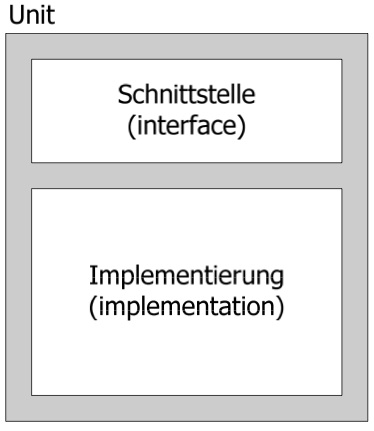
\includegraphics[width=0.28\textwidth]{pics/unit.jpg}
			\end{center}
	\end{minipage}

    \subsection{Die Schnittstellen-/Headerdatei \verweiscpp{10.3.1}}
		\begin{minipage}[t]{11 cm}
			 Jede .h-Datei enth�lt als erste Anweisungsfolge eine Include-Guard welche Mehrfacheinf�gen verhindert. Der Syntax lautet:
			 \lstinputlisting[language=C,tabsize=2]{code/includeguard.c}
			 Deklarationsreihenfolge in Headerdatei (*.h)  (Beispiel Kap 16.1)
			\begin{enumerate}
				\item Dateikommentar
				\item \#include der verwendeten System-Header (iostream, etc.) \newline
				      \#include <...>
				\item \#include der projektbezogenen Header (\#include "...")
				\item Konstantendefinitionen
				\item typedefs und Definition von Strukturen
				\item Allenfalls extern-Deklaration von globalen Variablen
				\item Funktionsprototypen, inkl. Kommentare der Schnittstelle, bzw. Klassendeklarationen
			\end{enumerate}
		\end{minipage}	
		\hspace*{0.5cm}
		\begin{minipage}[t]{7.5 cm}	
		  	\subsection{Beispiel Unit Rechteck}
		  	\lstinputlisting[language=c++,tabsize=2]{code/example_unit.cpp}
		\end{minipage}
\newpage
     	\begin{minipage}[t]{19 cm}
			\subsection{Die Implementierungsdatei \verweiscpp{10.3.2}}
				Deklarationsreihenfolge in Implementierungsdatei (*.cpp) (Beispiel Kap 16.1)
				\begin{enumerate}
			 		\item Dateikommentar
					\item \#include der verwendeten System-Header (iostream, etc.)
					      \#include <...>
					\item \#include der projektbezogenen Header (\#include "...") \newline
					      a) Hier k�me die Verwendung von $using$ $namespace$
					\item allenfalls globale Variablen und statische Variablen
					\item Pr�prozessor-Direktiven
					\item Funktionsprototypen von lokalen, internen Funktionen
					\item Definition von Funktionen und Klassen (Kommentare aus Headerdatei nicht wiederholen!!) 
					\linebreak
				\end{enumerate}
		\end{minipage}
		
		\subsection{Buildprozess / Makefile}
			\begin{minipage}[t]{11 cm}
			    Der Buildprozess erstellt aus den einzelnen Dateien einen ausf�hrbaren Code. Dazu werden zuerst alle *.cpp-Files compiliert.
			    Die daraus entstandenen Objektdatei m�ssen anschliessend gelinkt und somit zu einer auf�hrbaren Datei zusammengesetzt. Die Eingabe in der Konsole sieht wie folgt aus:
			    \lstinputlisting[language=C,tabsize=2]{code/compileUnit.c}
			    Es w�re m�hsam, wenn diese Befehle jedesmal neu eingetippt werden m�ssten. Deshalb wird in der Praxis oft ein Buildtool eingesetzt, z.B. make 
			 	\subsubsection{Make-File}
			 	\begin{compactitem}	
			 		\item In einem make-File k�nnen Abh�ngigkeiten definiert werden
			 		\item  Wenn eine Datei ge�ndert wurde, dann werden alle Operationen ausgef�hrt mit den Dateien, welche von dieser ge�nderten Datei abh�ngen
			 		\item Der Befehl (g++) wird z.B. nur dann ausgef�hrt, wenn sich an den Dateien, zu denen eine Abh�ngigkeit besteht, etwas ge�ndert hat
			 		\linebreak
				\end{compactitem}
				
			\end{minipage}
			\hspace*{0.5cm}
			\begin{minipage}[t]{7.5 cm}
				Abh�ngigkeitsliste gem�ss  UML-Notation:
				\linebreak
				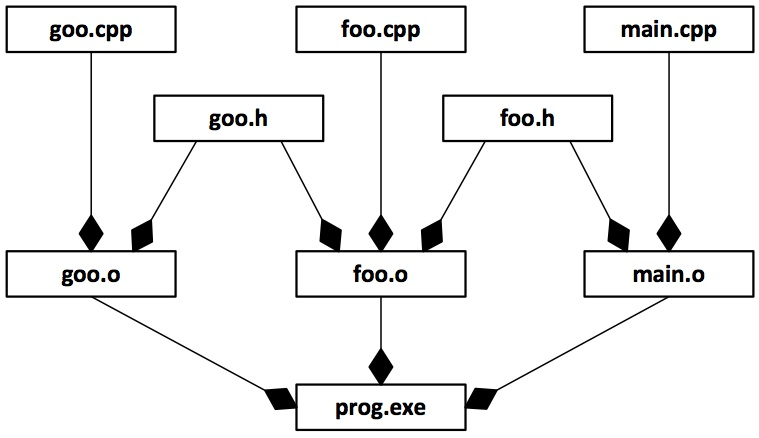
\includegraphics[width=1\textwidth]{pics/abhaengigkeitUML.jpg}
			    
			\end{minipage}
			\begin{minipage}[t]{19 cm}
			    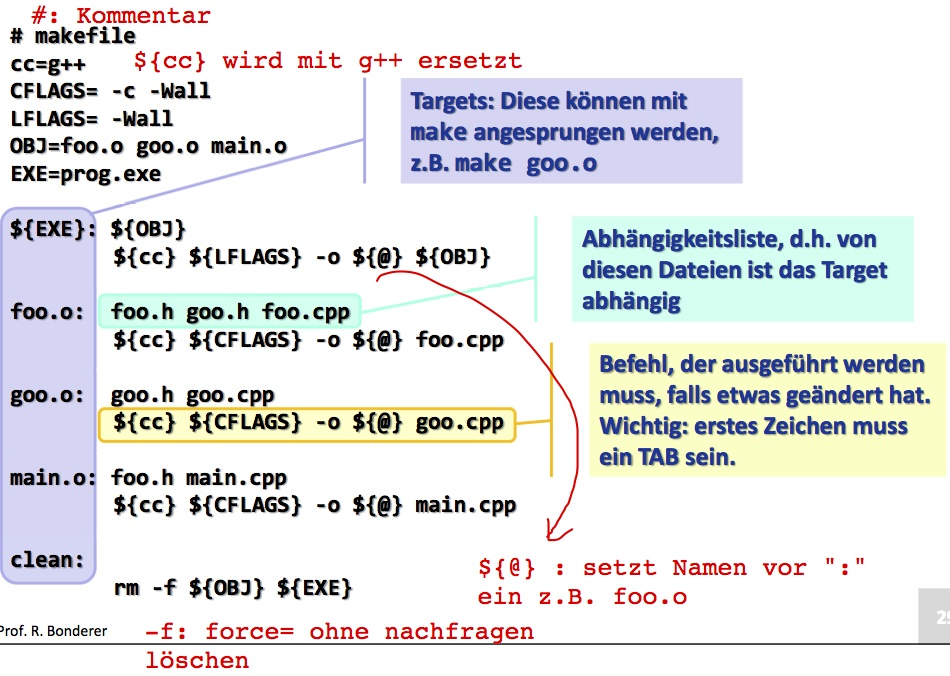
\includegraphics[width=0.6\textwidth]{pics/makefile.jpg}
			\end{minipage}
		
		
